
\documentclass[../capitulos/cap1.tex]{subfiles}

\tikzset{every picture/.style={line width=0.75pt}} %set default line width to 0.75pt

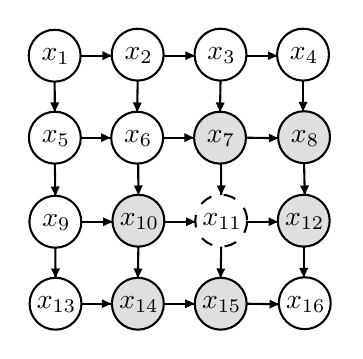
\begin{tikzpicture}[x=0.75pt,y=0.75pt,yscale=-0.5,xscale=0.5]
%uncomment if require: \path (0,426); %set diagram left start at 0, and has height of 426

\draw    (45.2, 36.5) circle [x radius= 25, y radius= 25]  ;
\draw    (125.2, 35.5) circle [x radius= 25, y radius= 25]  ;
\draw    (70.7,36.5) -- (100.2,36.5) ;
\draw [shift={(100.2,36.5)}, rotate = 180] [fill={rgb, 255:red, 0; green, 0; blue, 0 }  ] [draw opacity=0] (8.93,-4.29) -- (0,0) -- (8.93,4.29) -- (8.93,-4.29)    ;

\draw    (45.37, 115.5) circle [x radius= 25, y radius= 25]  ;
\draw    (124.7, 115.5) circle [x radius= 25, y radius= 25]  ;
\draw    (205.03, 35.5) circle [x radius= 25, y radius= 25]  ;
\draw    (284.53, 35.5) circle [x radius= 25, y radius= 25]  ;
\draw  [fill={rgb, 255:red, 225; green, 222; blue, 222 }  ,fill opacity=1 ]  (204.53, 115.5) circle [x radius= 25, y radius= 25]  ;
\draw  [fill={rgb, 255:red, 225; green, 222; blue, 222 }  ,fill opacity=1 ]  (285.53, 115) circle [x radius= 25, y radius= 25]  ;
\draw    (205.03,60.5) -- (204.53,90.5) ;
\draw [shift={(204.53,90.5)}, rotate = 270.95] [fill={rgb, 255:red, 0; green, 0; blue, 0 }  ] [draw opacity=0] (8.93,-4.29) -- (0,0) -- (8.93,4.29) -- (8.93,-4.29)    ;

\draw    (45.2,61.5) -- (45.37,90.5) ;
\draw [shift={(45.37,90.5)}, rotate = 269.67] [fill={rgb, 255:red, 0; green, 0; blue, 0 }  ] [draw opacity=0] (8.93,-4.29) -- (0,0) -- (8.93,4.29) -- (8.93,-4.29)    ;

\draw    (45.37,140.5) -- (45.87,171.5) ;
\draw [shift={(45.87,171.5)}, rotate = 269.08] [fill={rgb, 255:red, 0; green, 0; blue, 0 }  ] [draw opacity=0] (8.93,-4.29) -- (0,0) -- (8.93,4.29) -- (8.93,-4.29)    ;

\draw    (70.37,115.5) -- (98.87,115.5) ;
\draw [shift={(98.87,115.5)}, rotate = 180] [fill={rgb, 255:red, 0; green, 0; blue, 0 }  ] [draw opacity=0] (8.93,-4.29) -- (0,0) -- (8.93,4.29) -- (8.93,-4.29)    ;

\draw    (150.53,36.5) -- (180.03,36.5) ;
\draw [shift={(180.03,36.5)}, rotate = 180] [fill={rgb, 255:red, 0; green, 0; blue, 0 }  ] [draw opacity=0] (8.93,-4.29) -- (0,0) -- (8.93,4.29) -- (8.93,-4.29)    ;

\draw    (230.03,36.5) -- (259.53,36.5) ;
\draw [shift={(259.53,36.5)}, rotate = 180] [fill={rgb, 255:red, 0; green, 0; blue, 0 }  ] [draw opacity=0] (8.93,-4.29) -- (0,0) -- (8.93,4.29) -- (8.93,-4.29)    ;

\draw    (149.7,115.5) -- (179.2,115.5) ;
\draw [shift={(179.2,115.5)}, rotate = 180] [fill={rgb, 255:red, 0; green, 0; blue, 0 }  ] [draw opacity=0] (8.93,-4.29) -- (0,0) -- (8.93,4.29) -- (8.93,-4.29)    ;

\draw    (125.2,60.5) -- (124.7,90.5) ;
\draw [shift={(124.7,90.5)}, rotate = 270.95] [fill={rgb, 255:red, 0; green, 0; blue, 0 }  ] [draw opacity=0] (8.93,-4.29) -- (0,0) -- (8.93,4.29) -- (8.93,-4.29)    ;

\draw    (284.53,60.5) -- (284.53,90) ;
\draw [shift={(284.53,90)}, rotate = 270] [fill={rgb, 255:red, 0; green, 0; blue, 0 }  ] [draw opacity=0] (8.93,-4.29) -- (0,0) -- (8.93,4.29) -- (8.93,-4.29)    ;

\draw    (229.53,115.5) -- (260.53,116) ;
\draw [shift={(260.53,116)}, rotate = 180.92] [fill={rgb, 255:red, 0; green, 0; blue, 0 }  ] [draw opacity=0] (8.93,-4.29) -- (0,0) -- (8.93,4.29) -- (8.93,-4.29)    ;

\draw    (45.87, 196.5) circle [x radius= 25, y radius= 25]  ;
\draw  [fill={rgb, 255:red, 225; green, 222; blue, 222 }  ,fill opacity=1 ]  (125.87, 195.5) circle [x radius= 25, y radius= 25]  ;
\draw    (71.37,196.5) -- (100.87,196.5) ;
\draw [shift={(100.87,196.5)}, rotate = 180] [fill={rgb, 255:red, 0; green, 0; blue, 0 }  ] [draw opacity=0] (8.93,-4.29) -- (0,0) -- (8.93,4.29) -- (8.93,-4.29)    ;

\draw    (46.03, 275.5) circle [x radius= 25, y radius= 25]  ;
\draw  [fill={rgb, 255:red, 225; green, 222; blue, 222 }  ,fill opacity=1 ]  (125.37, 275.5) circle [x radius= 25, y radius= 25]  ;
\draw  [dash pattern={on 4.5pt off 4.5pt}]  (205.7, 195.5) circle [x radius= 25, y radius= 25]  ;
\draw  [fill={rgb, 255:red, 225; green, 222; blue, 222 }  ,fill opacity=1 ]  (285.2, 195.5) circle [x radius= 25, y radius= 25]  ;
\draw  [fill={rgb, 255:red, 225; green, 222; blue, 222 }  ,fill opacity=1 ]  (205.2, 275.5) circle [x radius= 25, y radius= 25]  ;
\draw    (286.2, 275) circle [x radius= 25, y radius= 25]  ;
\draw    (205.7,220.5) -- (205.2,250.5) ;
\draw [shift={(205.2,250.5)}, rotate = 270.95] [fill={rgb, 255:red, 0; green, 0; blue, 0 }  ] [draw opacity=0] (8.93,-4.29) -- (0,0) -- (8.93,4.29) -- (8.93,-4.29)    ;

\draw    (45.87,221.5) -- (46.03,250.5) ;
\draw [shift={(46.03,250.5)}, rotate = 269.67] [fill={rgb, 255:red, 0; green, 0; blue, 0 }  ] [draw opacity=0] (8.93,-4.29) -- (0,0) -- (8.93,4.29) -- (8.93,-4.29)    ;

\draw    (71.03,275.5) -- (99.53,275.5) ;
\draw [shift={(99.53,275.5)}, rotate = 180] [fill={rgb, 255:red, 0; green, 0; blue, 0 }  ] [draw opacity=0] (8.93,-4.29) -- (0,0) -- (8.93,4.29) -- (8.93,-4.29)    ;

\draw    (151.2,196.5) -- (180.7,196.5) ;
\draw [shift={(180.7,196.5)}, rotate = 180] [fill={rgb, 255:red, 0; green, 0; blue, 0 }  ] [draw opacity=0] (8.93,-4.29) -- (0,0) -- (8.93,4.29) -- (8.93,-4.29)    ;

\draw    (230.7,196.5) -- (260.2,196.5) ;
\draw [shift={(260.2,196.5)}, rotate = 180] [fill={rgb, 255:red, 0; green, 0; blue, 0 }  ] [draw opacity=0] (8.93,-4.29) -- (0,0) -- (8.93,4.29) -- (8.93,-4.29)    ;

\draw    (150.37,275.5) -- (179.87,275.5) ;
\draw [shift={(179.87,275.5)}, rotate = 180] [fill={rgb, 255:red, 0; green, 0; blue, 0 }  ] [draw opacity=0] (8.93,-4.29) -- (0,0) -- (8.93,4.29) -- (8.93,-4.29)    ;

\draw    (125.87,220.5) -- (125.37,250.5) ;
\draw [shift={(125.37,250.5)}, rotate = 270.95] [fill={rgb, 255:red, 0; green, 0; blue, 0 }  ] [draw opacity=0] (8.93,-4.29) -- (0,0) -- (8.93,4.29) -- (8.93,-4.29)    ;

\draw    (285.2,220.5) -- (285.2,250) ;
\draw [shift={(285.2,250)}, rotate = 270] [fill={rgb, 255:red, 0; green, 0; blue, 0 }  ] [draw opacity=0] (8.93,-4.29) -- (0,0) -- (8.93,4.29) -- (8.93,-4.29)    ;

\draw    (230.2,275.5) -- (261.2,276) ;
\draw [shift={(261.2,276)}, rotate = 180.92] [fill={rgb, 255:red, 0; green, 0; blue, 0 }  ] [draw opacity=0] (8.93,-4.29) -- (0,0) -- (8.93,4.29) -- (8.93,-4.29)    ;

\draw    (125.7,140.5) -- (125.87,170.5) ;
\draw [shift={(125.87,170.5)}, rotate = 269.68] [fill={rgb, 255:red, 0; green, 0; blue, 0 }  ] [draw opacity=0] (8.93,-4.29) -- (0,0) -- (8.93,4.29) -- (8.93,-4.29)    ;

\draw    (285.53,140) -- (286.2,170.5) ;
\draw [shift={(286.2,170.5)}, rotate = 268.75] [fill={rgb, 255:red, 0; green, 0; blue, 0 }  ] [draw opacity=0] (8.93,-4.29) -- (0,0) -- (8.93,4.29) -- (8.93,-4.29)    ;

\draw    (205.53,140.5) -- (205.7,170.5) ;
\draw [shift={(205.7,170.5)}, rotate = 269.68] [fill={rgb, 255:red, 0; green, 0; blue, 0 }  ] [draw opacity=0] (8.93,-4.29) -- (0,0) -- (8.93,4.29) -- (8.93,-4.29)    ;


\draw (46.2,37.44) node   {$x_{1}$};
\draw (126.2,36.44) node   {$x_{2}$};
\draw (46.37,116.44) node   {$x_{5}$};
\draw (125.7,116.44) node   {$x_{6}$};
\draw (206.03,36.44) node   {$x_{3}$};
\draw (285.53,36.44) node   {$x_{4}$};
\draw (205.53,116.44) node   {$x_{7}$};
\draw (286.53,115.94) node   {$x_{8}$};
\draw (46.87,197.44) node   {$x_{9}$};
\draw (126.87,196.44) node   {$x_{10}$};
\draw (47.03,276.44) node   {$x_{13}$};
\draw (126.37,276.44) node   {$x_{14}$};
\draw (206.7,196.44) node   {$x_{11}$};
\draw (286.2,196.44) node   {$x_{12}$};
\draw (206.2,276.44) node   {$x_{15}$};
\draw (287.2,275.94) node   {$x_{16}$};


\end{tikzpicture}
